% UVCC Phase 6 Native Parallelism (IEEE format)
\documentclass[10pt,conference]{IEEEtran}
\IEEEoverridecommandlockouts
\usepackage{amsmath,amssymb}
\usepackage{graphicx}
\usepackage{booktabs}
\usepackage{url}
\usepackage{hyperref}
\usepackage{xcolor}
\usepackage{listings}
\usepackage{tikz}
\usetikzlibrary{decorations.pathreplacing,arrows.meta,positioning,calc}
\lstset{basicstyle=\ttfamily\footnotesize,breaklines=true}
\hypersetup{colorlinks=true,linkcolor=blue,citecolor=blue,urlcolor=blue}

\title{UVCC Phase 6: Private, Verifiable, Fully-Parallel GPU Computation across Untrusted Domains}
\author{
  \IEEEauthorblockN{Alien Team}
  \IEEEauthorblockA{\texttt{research@uvcc.example}}
}

\begin{document}
\maketitle

\begin{abstract}
We present UVCC (Universal Verifiable Confidential Computing), a system that enables private and verifiable GPU computation across mutually distrustful domains. UVCC combines three-party replicated secret sharing (RSS) for confidentiality, a deterministic transcript-of-transcripts construction for verifiability, and native ML parallelism (DP/PP/TP) realized in a C++ GPU runtime with NCCL-based collectives and an exactly-once transport. We report a complete Phase~6 bring-up, diagnose and fix a PP deadlock, and demonstrate a large-scale run ($R{=}8,S{=}4,T{=}2,M{=}32$; 192 workers) with a determinism proof via matching global roots across reruns. We release a comprehensive, auditor-friendly log bundle along with scripts to derive metrics and figures directly from raw logs.
\end{abstract}

\section{Introduction}
Confidential and verifiable ML across providers requires both a privacy contract and a verifiable execution story without sacrificing parallel performance. UVCC delivers this by:
\begin{itemize}
  \item Confidentiality via three-party RSS (honest-majority).
  \item Verifiability via deterministic transcripts, subsession/replica/global roots, and an audit bundle.
  \item Native parallelism: DP, PP, TP on GPUs with robust NCCL initialization across heterogeneous infrastructure.
\end{itemize}

\section{Model and Guarantees}
Adversary corrupts at most one party. Secrets include inputs, weights, gradients, optimizer state, and intermediate values. Verifiability binds all protocol events into deterministic roots with canonical ordering. The audit bundle encodes subsession, replica, and global roots and is verified against identities and policy.

\section{System Overview}
UVCC consists of:
\begin{itemize}
  \item A reliable transport (exactly-once frame acceptance with conservative retries and long-polling).
  \item A transcript store (deterministic hashing, versioned leaf prefixes, Merkle roots).
  \item A native runtime integrating OPEN/LIFT engines and NCCL collectives for DP/PP/TP.
\end{itemize}
The Phase~6 worker executes a 1F1B-style schedule with careful PP/DP/NCCL ordering to avoid deadlocks.

\begin{figure}[t]
  \centering
  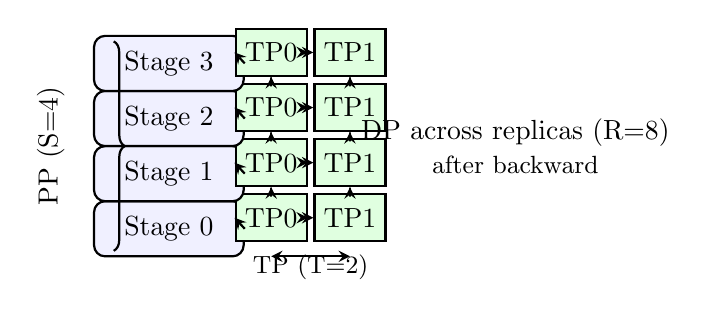
\begin{tikzpicture}[x=1.0cm,y=0.7cm,>=stealth,thick]
    \foreach \s in {0,...,3} {
      \node[draw,rounded corners,minimum width=1.9cm,minimum height=0.7cm,fill=blue!6] (stage\s) at (0,\s) {Stage \s};
      \node[draw,minimum width=0.9cm,minimum height=0.6cm,fill=green!12] (tpA\s) at (1.3,\s+0.2) {TP0};
      \node[draw,minimum width=0.9cm,minimum height=0.6cm,fill=green!12] (tpB\s) at (2.3,\s+0.2) {TP1};
      \draw[->] (stage\s.east) -- (tpA\s.west);
      \draw[<->,densely dashed] (tpA\s.east) -- (tpB\s.west);
    }
    \foreach \s in {0,...,2} {
      \draw[->] (tpA\s.north) .. controls +(0,0.3) and +(0,-0.3) .. (tpA\the\numexpr\s+1\relax.south);
      \draw[->] (tpB\s.north) .. controls +(0,0.3) and +(0,-0.3) .. (tpB\the\numexpr\s+1\relax.south);
    }
    \draw[decorate,decoration={brace,amplitude=4pt,mirror}] (-0.7,-0.4) -- (-0.7,3.4) node[midway,xshift=-0.8cm,rotate=90] {PP (S=4)};
    \node at (1.8,-0.7) {\small TP (T=2)};
    \draw[<->] (1.3,-0.5) -- (2.3,-0.5);
    \node[align=center] at (4.4,1.5) {DP across replicas (R=8)\\\small after backward};
  \end{tikzpicture}
  \caption{Native parallelism: PP across stages, TP within stage, DP across replicas.}
  \label{fig:topology}
\end{figure}

\section{Implementation Highlights}
\textbf{Transport.} Exactly-once receive with retransmit/backoff; long timeouts and long-polling reduce overload and tolerate party skew.
\textbf{NCCL.} Robust UID distribution and timeout control via \texttt{--phase6-timeout-s}; NCCL Socket NET across VMs; deterministic group construction.
\textbf{Scheduler.} PP gradient recvs posted per microbatch to avoid single-stream deadlock; DP init delayed until after backward to avoid OPEN skew.

\section{Evaluation}
\subsection{Setup}
We launch on 24 pods spanning providers. Final run topology: R=8, S=4, T=2, M=32 (192 workers). Logs are consolidated into a single explained file; our scripts derive metrics and figures from those logs for reproducibility.

\subsection{NCCL Initialization Metrics}
\begin{figure}[t]
  \centering
  \includegraphics[width=\linewidth]{figs/nccl_init_hist.png}
  \caption{NCCL init time distribution by nranks (TP=2, PP=4, DP=8).}
  \label{fig:nccl-hist}
\end{figure}
\begin{figure}[t]
  \centering
  \includegraphics[width=\linewidth]{figs/nccl_init_cdf.png}
  \caption{NCCL init time CDF by group type (TP/PP/DP).}
  \label{fig:nccl-cdf}
\end{figure}

\subsection{Protocol Event Coverage}
\begin{figure}[t]
  \centering
  \includegraphics[width=\linewidth]{figs/event_counts.png}
  \caption{Phase 6 event counts (epoch roots, OPEN completions, DP readiness).}
  \label{fig:event-counts}
\end{figure}
\begin{figure}[t]
  \centering
  \includegraphics[width=\linewidth]{figs/dp_ready_heatmap.png}
  \caption{DP readiness fraction per (stage s, tensor rank t), annotated as \texttt{ready/expected}. Uniform color indicates complete DP readiness.}
  \label{fig:dp-heat}
\end{figure}

\begin{figure}[t]
  \centering
  \includegraphics[width=\linewidth]{figs/dp_init_p50_heatmap.png}
  \caption{DP NCCL init latency p50 per (stage s, tensor rank t).}
  \label{fig:dp-init-heat}
\end{figure}

\subsection{Robustness Indicators}
\begin{figure}[t]
  \centering
  \includegraphics[width=\linewidth]{figs/error_counts.png}
  \caption{Robustness indicators (final run): worker timeouts and transport aborts are zero; runner SSH banner errors occurred during artifact collection and were tolerated.}
  \label{fig:error-counts}
\end{figure}
\begin{figure}[t]
  \centering
  \includegraphics[width=\linewidth]{figs/errors_by_group.png}
  \caption{Errors partitioned by group (TP/PP/DP) and type.}
  \label{fig:errors-by-group}
\end{figure}

\subsection{Determinism Proof}
We ran the full job twice with fixed \texttt{sid\_job\_hex}; the resulting \texttt{global\_root\_hex} values matched exactly, demonstrating determinism under cross-provider skew.

\section{Related Work}
We build on MPC, verifiable computation, and large-scale ML parallelism; UVCC’s novelty is an auditor-grade verifiable MPC runtime with native DP/PP/TP across domains.

\section{Conclusion}
UVCC Phase~6 demonstrates that private, verifiable, fully-parallel GPU computation across untrusted domains is practical and deterministic at scale. Future work: GPU-accelerated preprocessing (TCF/W-VOLE), production SKS, and larger model pipelines.

\section*{Artifacts and Reproducibility}
Figures are generated by \texttt{research/uvcc\_native/scripts/make\_phase6\_figs.py} from the consolidated log:
\newline\texttt{research/uvcc\_native/out-.../all\_logs\_explained.md}.

\end{document}


